\documentclass{article}

\usepackage{amsmath,amssymb,amsthm, amsfonts, palatino, mathpazo, array}
\usepackage{minted}
\newcommand\bmatr[1]{\begin{bmatrix} #1\end{bmatrix}}
\newcommand\dd{\text{d}\;}
\newcommand\p[2]{\frac{\partial #1}{\partial #2}}
\newcommand\inv[1]{\frac{1}{#1}}

\usepackage{hyperref}
\usepackage[margin=2.0cm]{geometry}

\usepackage{graphicx}
\graphicspath{ {/home/ubuntu/www/octopress/source/} }
\setlength{\parindent}{1cm}
\newgeometry{left=1.4in,right=1.4in, top=0.6in, bottom=0.6in}
\author{Andrew Gibiansky}
\date{\today}
\def\title{Quadcopter Dynamics, Simulation, and Control}

\begin{document}

\section*{Introduction}
A helicopter is a flying vehicle which uses rapidly spinning rotors to push air downwards, thus
creating a thrust force keeping the helicopter aloft. Conventional helicopters have two rotors.
These can be arranged as two coplanar rotors both providing upwards thrust, but spinning in opposite
directions (in order to balance the torques exerted upon the body of the helicopter). The two rotors
can also be arranged with one main rotor providing thrust and a smaller side rotor oriented
laterally and counteracting the torque produced by the main rotor. However, these configurations
require complicated machinery to control the direction of motion; a swashplate is used to change the
angle of attack on the main rotors. In order to produce a torque the angle of attack is modulated by
the location of each rotor in each stroke, such that more thrust is produced on one side of the
rotor plane than the other. The complicated design of the rotor and swashplate mechanism presents
some problems, increasing construction costs and design complexity.

A quadrotor helicopter (quadcopter) is a helicopter which has four equally spaced rotors, usually
arranged at the corners of a square body. With four independent rotors, the need for a swashplate
mechanism is alleviated. The swashplate mechanism was needed to allow the helicopter to utilize more
degrees of freedom, but the same level of control can be obtained by adding two more rotors.


The development of quadcopters has stalled until very recently, because controlling four independent
rotors has proven to be incredibly difficult and impossible without electronic assistance. The
decreasing cost of modern microprocessors has made electronic and even completely autonomous control
of quadcopters feasible for commercial, military, and even hobbyist purposes.

Quadcopter control is a fundamentally difficult and interesting problem. With six degrees of freedom
(three translational and three rotational) and only four independent inputs (rotor speeds),
quadcopters are severely underactuated. In order to achieve six degrees of freedom, rotational and
translational motion are coupled. The resulting dynamics are highly nonlinear, especially after
accounting for the complicated aerodynamic effects. Finally, unlike ground
vehicles, helicopters have very little friction to prevent their motion, so they must provide their
own damping in order to stop moving and remain stable. Together, these factors create a very
interesting control problem. We will present a very simplified model of quadcopter dynamics and
design controllers for our dynamics to follow a designated trajectory. We will then test our
controllers with a numerical simulation of a quadcopter in flight.

\newpage
\section*{Quadcopter Dynamics}
We will start deriving quadcopter dynamics by introducing the two frames in which will operate. The
inertial frame is defined by the ground, with gravity pointing in the negative $z$ direction. The
body frame is defined by the orientation of the quadcopter, with the rotor axes pointing in the
positive $z$ direction and the arms pointing in the $x$ and $y$ directions.
\begin{center}
    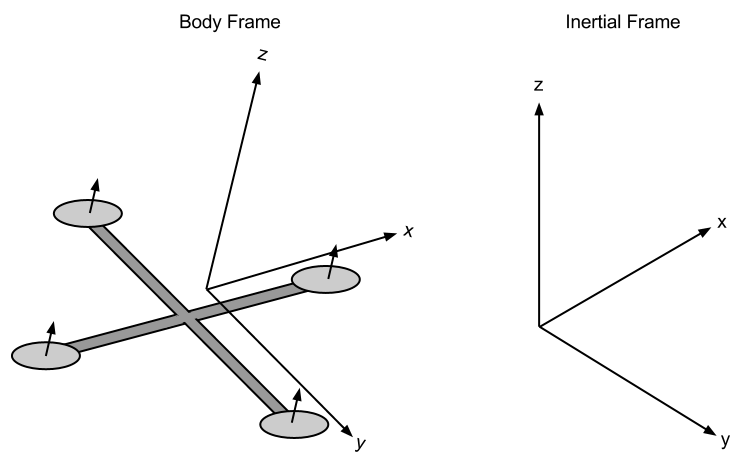
\includegraphics[scale=0.3]{images/Quadcopter_Coordinates.png} \\
    {Quadcopter Body Frame and Inertial Frame}
\end{center}

\subsection*{Kinematics}
Before delving into the physics of quadcopter motion, let us formalize the kinematics in the body
and inertial frames. We define the position and velocity of the quadcopter in the inertial frame as
$x = ({x , y , z})^T$ and $\dot x = ({\dot x , \dot y , \dot z})^T$, respectively.
Similarly, we define the roll, pitch, and yaw angles in the body frame as
$\theta = ({\phi , \theta , \psi})^T$, with corresponding angular velocities equal to
$\dot \theta =  ({\dot \phi , \dot \theta , \dot \psi})^T$.
However, note that the angular velocity vector $\omega \ne \dot \theta$. The angular velocity is a vector
pointing along the axis of rotation, while $\dot \theta$ is just the time derivative of yaw, pitch,
and roll.  In order to convert these angular velocities into the angular velocity vector, we can use
the following relation:
\[\omega = \bmatr{
    1 &0 & -s_\theta \\
    0 & c_\phi & c_\theta s_\phi \\
    0 & -s_\phi & c_\theta c_\phi
} \dot\theta\]
where $\omega$ is the angular velocity vector in the body frame.

We can relate the body and inertial frame by a rotation matrix $R$ which goes from the body frame to
the inertial frame. This matrix is derived by using the ZYZ Euler angle conventions and successively
``undoing'' the yaw, pitch, and roll.
\[R = \bmatr{
    c_\phi  c_\psi - c_\theta  s_\phi  s_\psi &  -c_\psi  s_\phi -  c_\phi  c_\theta  s_\psi &  s_\theta  s_\psi\\
    c_\theta  c_\psi  s_\phi + c_\phi  s_\psi &  c_\phi  c_\theta  c_\psi - s_\phi  s_\psi &  -c_\psi  s_\theta\\
    s_\phi  s_\theta &  c_\phi  s_\theta &  c_\theta\\
}\]
For a given vector $\vec v$ in the body frame, the corresponding vector is given by $R\vec v$ in the
inertial frame.

\subsection*{Physics}
In order to properly model the dynamics of the system, we need an understanding of the physical
properties that govern it. We will begin with a description of the motors being used for our
quadcopter, and then use energy considerations to derive the forces and thrusts that these motors
produce on the entire quadcopter. All motors on the quadcopter are identical, so we can analyze a
single one without loss of generality. Note that adjacent propellers, however, are oriented opposite
each other; if a propeller is spinning ``clockwise'', then the two adjacent ones will be spinning
``counter-clockwise'', so that torques are balanced if all propellers are spinning at the same rate.
\subsubsection*{Motors}
Brushless motors are used for all quadcopter applications. For our electric motors, the torque
produced is given by
\[\tau = K_t (I - I_0)\]
where $\tau$ is the motor torque, $I$ is the input current, $I_0$ is the current when there is no
load on the motor, and $K_t$ is the torque proportionality constant. The voltage across the motor is
the sum of the back-EMF and some resistive loss:
\[V = I R_m  + K_v \omega\]
where $V$ is the voltage drop across the motor, $R_m$ is the motor resistance, $\omega$ is the
angular velocity of the motor, and $K_v$ is a proportionality constant (indicating back-EMF
generated per RPM).
We can use this description of our motor to calculate the power it consumes. The power is
\[P = IV = \frac{(\tau + K_t I_0) (K_t I_0 R_m + \tau R_m + K_t K_v \omega)}{ {K_t}^2}\]
For the purposes of our simple model, we will assume a negligible motor resistance. Then, the power
becomes proportional to the angular velocity:
\[P \approx \frac{(\tau + K_t I_0)  K_v \omega}{ {K_t}}\]
Further simplifying our model, we assume that $K_t I_0 \ll \tau$. This is not altogether unreasonable,
since $I_0$ is the current when there is no load, and is thus rather small. In practice, this
approximation holds well enough. Thus, we obtain our final, simplified equation for power:
\[P \approx \frac{K_v}{K_t} \tau \omega.\]
\subsubsection*{Forces}
The power is used to keep the quadcopter aloft. By conservation of energy, we know that the 
energy the motor expends in a given time period is equal to the force generated on the propeller
times the distance that the air it displaces moves ($P\cdot \dd t = F \cdot \dd x$). Equivalently, the \emph{power} is equal to the
thrust times the air velocity ($P = F\frac{\dd x}{\dd t}$).
\[P = Tv_h\]
We assume vehicle speeds are low, so $v_h$ is the air velocity when hovering. We also assume that
the free stream velocity, $v_\infty$, is zero (the air in the surrounding environment is stationary
relative to the quadcopter). Momentum theory gives us the equation for hover
velocity as a function of thrust,
\[v_h = \sqrt\frac{T}{2\rho A}\]
where $\rho$ is the density of the surrounding air and $A$ is the area swept out by the rotor. Using
our simplified equation for power, we can then write
\[P = \frac{K_v}{K_t} \tau \omega = \frac{K_vK_\tau}{K_t} T \omega = \frac{T^\frac{3}{2}}{\sqrt{2\rho A}}.\]
Note that in the general case, $\tau = \vec r \times \vec F$; in this case, the torque is
proportional to the thrust $T$ by some constant ratio $K_\tau$ determined by the blade configuration
and parameters. Solving for the thrust magnitude $T$, 
we obtain that thrust is proportional to the square of angular velocity of the motor:
\[T = \left(\frac{K_vK_\tau\sqrt{2 \rho A}}{K_t} \omega\right)^2 = k\omega^2\]
where $k$ is some appropriately dimensioned constant. Summing over all the motors, 
we find that the total thrust on the quadcopter (in the body frame) is given by
\[T_B = \sum_{i=1}^4 T_i = k\bmatr{ 0 \\ 0 \\ \sum {\omega_i}^2 }.\]

In addition to the thrust force, we will model friction as a force proportional to the linear
velocity in each direction. This is a highly simplified view of fluid friction, but will be
sufficient for our modeling and simulation. Our global drag forces will be modeled by an additional
force term
\[F_D = \bmatr{
    -k_d\dot x \\
    -k_d\dot y \\
    -k_d\dot z \\
}\]
If additional precision is desired, the constant $k_d$ can be separated into three separate friction
constants, one for each direction of motion. If we were to do this, we would want to model friction
in the body frame rather than the inertial frame.

\subsubsection*{Torques}
Now that we have computed the forces on the quadcopter, we would also like to compute the torques.
Each rotor contributes some torque about the body $z$ axis. This torque is the torque required to
keep the propeller spinning and providing thrust; it creates the instantaneous angular acceleration
and overcomes the frictional drag forces. The drag equation from fluid dynamics gives us the
frictional \emph{force}:
\[F_D = \frac{1}{2}\rho C_D A v^2.\]
where $\rho$ is the surrounding fluid density, $A$ is the reference area (propeller cross-section,
\emph{not} area swept out by the propeller),
and $C_D$ is a dimensionless constant. This, while only accurate in some in some cases, is good
enough for our purposes. This implies that the torque due to drag is given by
\[\tau_D = \frac{1}{2}R \rho C_D A v^2 = \frac{1}{2}R \rho C_D A (\omega R)^2 = b\omega^2\]
where $\omega$ is the angular velocity of the propeller, $R$ is the radius of the propeller, and $b$
is some appropriately dimensioned constant. Note
that we've assumed that all the force is applied at the tip of the propeller, which is certainly
inaccurate; however, the only result that matters for our purposes is that the drag torque is proportional to the
square of the angular velocity. We can then write the complete torque about the $z$ axis for the
$i$th motor:
\[\tau_z = b\omega^2 + I_M \dot\omega\]
where $I_M$ is the moment of inertia about the motor $z$ axis, $\dot\omega$ is the angular
acceleration of the propeller, and $b$ is our drag coefficient. Note that in steady state flight
(i.e. not takeoff or landing), $\dot\omega \approx 0$, since most of the time the propellers will be
maintaining a constant (or almost constant) thrust and won't be accelerating. Thus, we ignore this
term, simplifying the entire expression to
\[\tau_z = (-1)^{i+1} b{\omega_i}^2.\]
where the $(-1)^{i+1}$ term is positive for the $i$th propeller if the propeller is spinning clockwise
and negative if it is spinning counterclockwise. The total torque about the $z$ axis is given by the
sum of all the torques from each propeller:
\[\tau_\psi = b\left( {\omega_1}^2 -  {\omega_2}^2 +  {\omega_3}^2 -  {\omega_4}^2\right)\]
The roll and pitch torques are derived from standard mechanics. We can arbitrarily choose the $i =
1$ and $i=3$ motors to be on the roll axis, so
\[\tau_\phi = \sum r\times T = L(k{\omega_1}^2 - k{\omega_3}^2) = Lk({\omega_1}^2 - {\omega_3}^2)\]
Correspondingly, the pitch torque is given by a similar expression
\[\tau_\theta = Lk({\omega_2}^2 - {\omega_4}^2)\]
where $L$ is the distance from the center of the quadcopter to any of the propellers. All together,
we find that the torques in the body frame are
\[\tau_B = \bmatr{
    Lk({\omega_1}^2 - {\omega_3}^2) \\
    Lk({\omega_2}^2 - {\omega_4}^2) \\
    b\left( {\omega_1}^2 -  {\omega_2}^2 +  {\omega_3}^2 -  {\omega_4}^2\right)
}\]

The model we've derived so far is highly simplified. We ignore a multitude of advanced effects that
contribute to the highly nonlinear dynamics of a quadcopter. We ignore rotational drag forces (our rotational velocities are relatively low),
blade flapping (deformation of propeller blades due to high velocities and flexible materials), surrounding fluid velocities (wind), etc.
With that said, we now have all the parts necessary to write out the dynamics of our quadcopter.

\subsubsection*{Equations of Motion}
In the inertial frame, the acceleration of the quadcopter is due to thrust, gravity, and linear
friction. We can obtain the thrust vector in the inertial frame by using our rotation matrix $R$ to
map the thrust vector from the body frame to the inertial frame. Thus, the linear motion can be
summarized as
\[m\ddot{x} = \bmatr{0 \\ 0 \\ -mg} + RT_B + F_D\]
where $\vec x$ is the position of the quadcopter, $g$ is the acceleration due to gravity, $F_D$ is
the drag force, and $T_B$ is the thrust vector in the body frame. 
%
%We can also write these equations
%in the body frame, in which case we need to account for centripetal forces:
%\[m\ddot{x} = R^{-1}\bmatr{0 \\ 0 \\ -mg} + T_B + R^{-1}F_D - \omega\times(m\dot x)\]
%We can simplify this and simply omit the $R^{-1}$ term in the frictional forces, because there is
%nothing physically special about frictional forces in the inertial versus body frames. 

While it is convenient to have the linear equations of
motion in the inertial frame, the rotational equations of motion are useful to us in the body frame,
so that we can express rotations about the center of the quadcopter instead of about our inertial
center. We derive the rotational equations of motion from Euler's equations for rigid body dynamics. 
Expressed in vector form, Euler's equations are written as
\[I\dot\omega + \omega\times (I\omega) = \tau\]
where $\omega$ is the angular velocity vector, $I$ is the inertia matrix, and $\tau$ is a vector of
external torques. We can rewrite this as
\[ \dot\omega = \bmatr{\dot \omega_x \\ \dot \omega_y \\ \dot \omega_z} = I^{-1}\left(\tau - \omega\times (I\omega)\right).\]
We can model our quadcopter as two thin uniform rods crossed at the origin with a point mass (motor)
at the end of each. With this in mind, it's clear that the symmetries result in a diagonal inertia
matrix of the form
\[I = \bmatr{I_{xx} & 0 & 0 \\ 0 & I_{yy} & 0 \\ 0 & 0 & I_{zz}}.\]
Therefore, we obtain our final result for the body frame rotational equations of motion
\[\dot\omega = \bmatr{
    \tau_\phi {I_{xx}}^{-1} \\
    \tau_\theta {I_{yy}}^{-1} \\
    \tau_\psi {I_{zz}}^{-1}
} - \bmatr{
    \frac{I_{yy} - I_{zz}}{I_{xx}} \omega_y\omega_z \\ 
    \frac{I_{zz} - I_{xx}}{I_{yy}} \omega_x\omega_z  \\
    \frac{I_{xx} - I_{yy}}{I_{zz}} \omega_x\omega_y
}\]

\section*{Simulation}
Now that we have complete equations of motion describing the dynamics of the system, we can create a
simulation environment in which to test and view the results of various inputs and controllers.
Although more advanced methods are available, we can quickly write a simulator which utilizes
Euler's method for solving differential equations to evolve the system state. In MATLAB, this
simulator would be written as follows.
\begin{minted}{matlab}
% Simulation times, in seconds.
start_time = 0;
end_time = 10;
dt = 0.005;
times = start_time:dt:end_time;

% Number of points in the simulation.
N = numel(times);

% Initial simulation state.
x = [0; 0; 10];
xdot = zeros(3, 1);
theta = zeros(3, 1);

% Simulate some disturbance in the angular velocity.
% The magnitude of the deviation is in radians / second.
deviation = 100;
thetadot = deg2rad(2 * deviation * rand(3, 1) - deviation);

% Step through the simulation, updating the state.
for t = times
    % Take input from our controller.
    i = input(t);

    omega = thetadot2omega(thetadot, theta);

    % Compute linear and angular accelerations.
    a = acceleration(i, theta, xdot, m, g, k, kd);
    omegadot = angular_acceleration(i, omega, I, L, b, k);

    omega = omega + dt * omegadot;
    thetadot = omega2thetadot(omega, theta); 
    theta = theta + dt * thetadot;
    xdot = xdot + dt * a;
    x = x + dt * xdot;
end
\end{minted}
We would then need functions to compute all of the physical forces and torques.
\begin{minted}{matlab}
% Compute thrust given current inputs and thrust coefficient.
function T = thrust(inputs, k)
    % Inputs are values for ${\omega_i}^2$
    T = [0; 0; k * sum(inputs)];
end

% Compute torques, given current inputs, length, drag coefficient, and thrust coefficient.
function tau = torques(inputs, L, b, k)
    % Inputs are values for ${\omega_i}^2$
    tau = [
        L * k * (inputs(1) - inputs(3))
        L * k * (inputs(2) - inputs(4))
        b * (inputs(1) - inputs(2) + inputs(3) - inputs(4))
    ];
end

function a = acceleration(inputs, angles, xdot, m, g, k, kd)
    gravity = [0; 0; -g];
    R = rotation(angles);
    T = R * thrust(inputs, k);
    Fd = -kd * xdot;
    a = gravity + 1 / m * T + Fd;
end

function omegadot = angular_acceleration(inputs, omega, I, L, b, k)
    tau = torques(inputs, L, b, k);
    omegaddot = inv(I) * (tau - cross(omega, I * omega));
end
\end{minted}
We would also need values for all of our physical constants, a function to compute the rotation
matrix $R$, and functions to convert from an angular velocity vector $\omega$ to the derivatives of
roll, pitch, and yaw and vice-versa. These are not shown. We can then draw the quadcopter in a
three-dimensional visualization which is updated as the simulation is running.
\begin{center}
    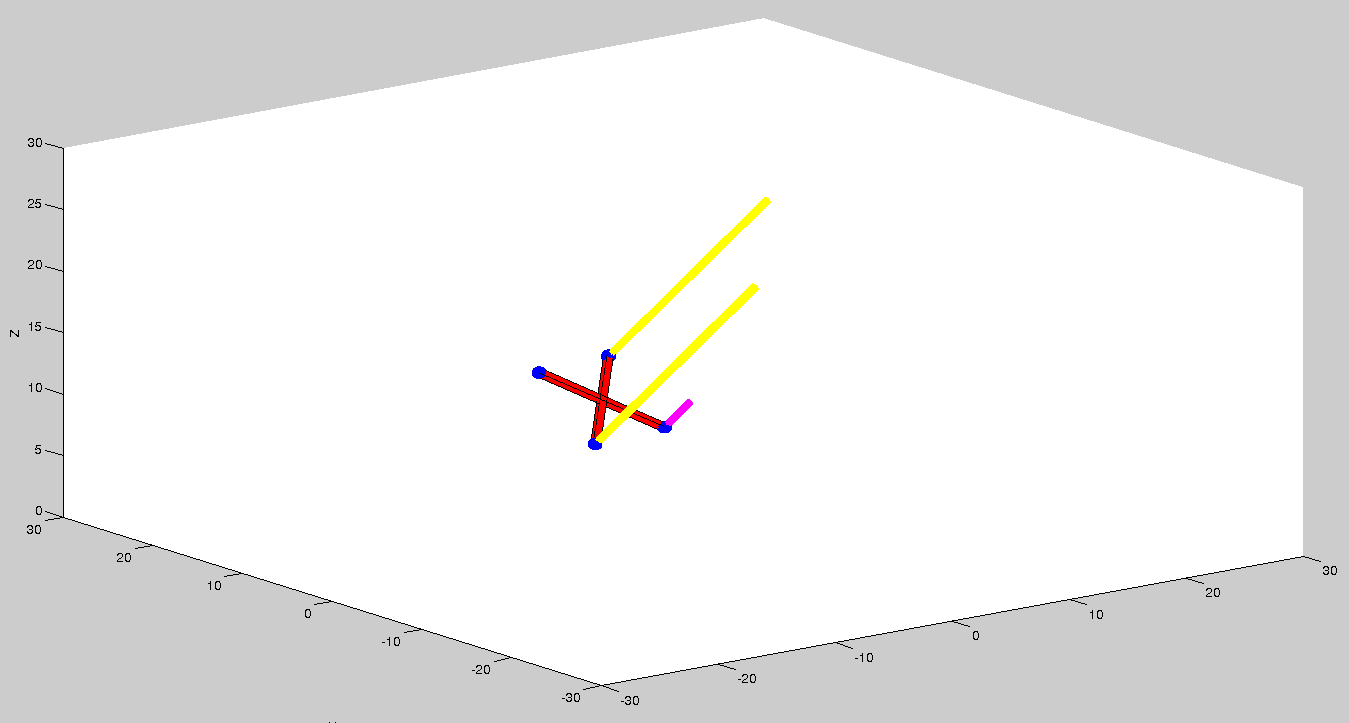
\includegraphics[scale=0.3]{images/simulation.png} \\
    {
        Quadcopter Simulation. Bars above each propeller represent, roughly, relative thrust magnitudes.
    }
\end{center}

\section*{Control}
The purpose of deriving a mathematical model of a quadcopter is to assist in developing controllers
for physical quadcopters. The inputs to our system consist of the angular velocities of each rotor,
since all we can control is the voltages across the
motors. Note that in our simplified model, we only use the square of the angular velocities,
${\omega_i}^2$, and never the angular velocity itself, $\omega_i$. For notational simplicity, let us
introduce the inputs $\gamma_i = {\omega_i}^2$. Since we can set $\omega_i$, we can
clearly set $\gamma_i$ as well. With this, we can write our system as a first order differential
equation in state space. Let $x_1$ be the position in space of the quadcopter, $x_2$ be the
quadcopter linear velocity, $x_3$ be the roll, pitch, and yaw angles, and $x_4$ be the angular
velocity vector. (Note that all of these are 3-vectors.) With these being our state, we can write
the state space equations for the evolution of our state.
\begin{align*}
    \dot{x_1} &= x_2 \\
    \dot{x_2} &= \bmatr{0 \\ 0 \\ -g} + \frac{1}{m} RT_B + \frac{1}{m} F_D \\
    \dot{x_3} &= \bmatr{
        1 &0 & -s_\theta \\
        0 & c_\phi & c_\theta s_\phi \\
        0 & -s_\phi & c_\theta c_\phi
    }^{-1} x_4 \\
    \dot{x_4} &=  \bmatr{
        \tau_\phi {I_{xx}}^{-1} \\
        \tau_\theta {I_{yy}}^{-1} \\
        \tau_\psi {I_{zz}}^{-1}
    } - \bmatr{
        \frac{I_{yy} - I_{zz}}{I_{xx}} \omega_y\omega_z \\ 
        \frac{I_{zz} - I_{xx}}{I_{yy}} \omega_x\omega_z  \\
        \frac{I_{xx} - I_{yy}}{I_{zz}} \omega_x\omega_y
    }
\end{align*}
Note that our inputs are not used in these equations directly. However, as we will see, we can
choose values for $\tau$ and $T$, and then solve for values of $\gamma_i$.

\subsection*{PD Control}
In order to control the quadcopter, we will use a PD control, with a component proportional to the
error between our desired trajectory and the observed trajectory, and a component proportional to
the derivative of the error. Our quadcopter will only have a gyro, so we will only be able to use the
angle derivatives $\dot\phi$, $\dot\theta$, and $\dot\psi$ in our controller; these measured values
will give us the derivative of our error, and their integral will provide us with the actual error. We would like to
stabilize the helicopter in a horizontal position, so our desired velocities and angles will all be
zero. Torques are related to our angular velocities by $\tau = I\ddot\theta$, so we would like to set the torques proportional to the
output of our controller, with $\tau = I u(t)$. Thus,
\[\bmatr{\tau_\phi \\ \tau_\theta \\ \tau_\psi} = \bmatr{
    -I_{xx} \left( K_d\dot\phi + K_p \int_0^T \dot\phi \dd t \right) \\
    -I_{yy} \left( K_d\dot\theta + K_p \int_0^T \dot\theta \dd t \right) \\
    -I_{zz} \left( K_d\dot\psi + K_p \int_0^T \dot\psi \dd t \right) \\
}\]
We have previously derived the relationship between torque and our inputs, so we know that
\[\tau_B = \bmatr{
    Lk({\gamma_1} - {\gamma_3}) \\
    Lk({\gamma_2} - {\gamma_4}) \\
    b\left( {\gamma_1} -  {\gamma_2} +  {\gamma_3} -  {\gamma_4}\right)
} = \bmatr{
    -I_{xx} \left( K_d\dot\phi + K_p \int_0^T \dot\phi \dd t \right) \\
    -I_{yy} \left( K_d\dot\theta + K_p \int_0^T \dot\theta \dd t \right) \\
    -I_{zz} \left( K_d\dot\psi + K_p \int_0^T \dot\psi \dd t \right) \\
}\]
This gives us a set of three equations with four unknowns. We can constrain this by enforcing the
constraint that our inputs must keep the quadcopter aloft:
\[T = mg.\]
Note that this equation ignores the fact that the thrust will not be pointed directly up. This will limit
the applicability of our controller, but should not cause major problems for small deviations from
stability. If we had a way of determining the current angle accurately, we could compensate.
If our gyro is precise enough, we can integrate the values obtained from the gyro to get the angles
$\theta$ and $\phi$. In this case, we can calculate the thrust necessary to keep the quadcopter
aloft by projecting the thrust $mg$ onto the inertial $z$ axis. We find that
\[T_\text{proj} = mg\cos\theta\cos\phi\]
Therefore, with a precise angle measurement, we can instead enforce the requirement that the thrust
be equal to
\[T = \frac{mg}{\cos\theta\cos\phi}\]
in which case the component of the thrust pointing along the positive $z$ axis will be equal to $mg$.
We know that the thrust is proportional to a weighted sum of the inputs:
\[T = \frac{mg}{\cos\theta\cos\phi} = k\sum \gamma_i \implies \sum\gamma_i = \frac{mg}{k\cos\theta\cos\phi}\]
With this extra constraint, we have a set of four linear equations with four unknowns $\gamma_i$. We
can then solve for each $\gamma_i$, and obtain the following input values:
\begin{align*}
    \gamma_1 &= \frac{mg}{4k\cos\theta\cos\phi}-\frac{2 b {e_\phi} {I_{xx}}+{e_\psi} {I_{zz}} k L}{4 b k L} \\
    \gamma_2 &= \frac{mg}{4k\cos\theta\cos\phi}+\frac{ {e_\psi} {I_{zz}}}{4 b}-\frac{ {e_\theta} {I_{yy}}}{2 k L} \\
    \gamma_3 &= \frac{mg}{4k\cos\theta\cos\phi}-\frac{-2 b {e_\phi} {I_{xx}}+{e_\psi} {I_{zz}} k L}{4 b k L} \\
    \gamma_4 &= \frac{mg}{4k\cos\theta\cos\phi}+\frac{ {e_\psi} {I_{zz}}}{4 b}+\frac{ {e_\theta} {I_{yy}}}{2 k L}
\end{align*}

This is a complete specification for our PD controller. We can simulate this controller using our simulation environment. 
The controller drives the angular velocities and angles to zero.
\begin{center}
    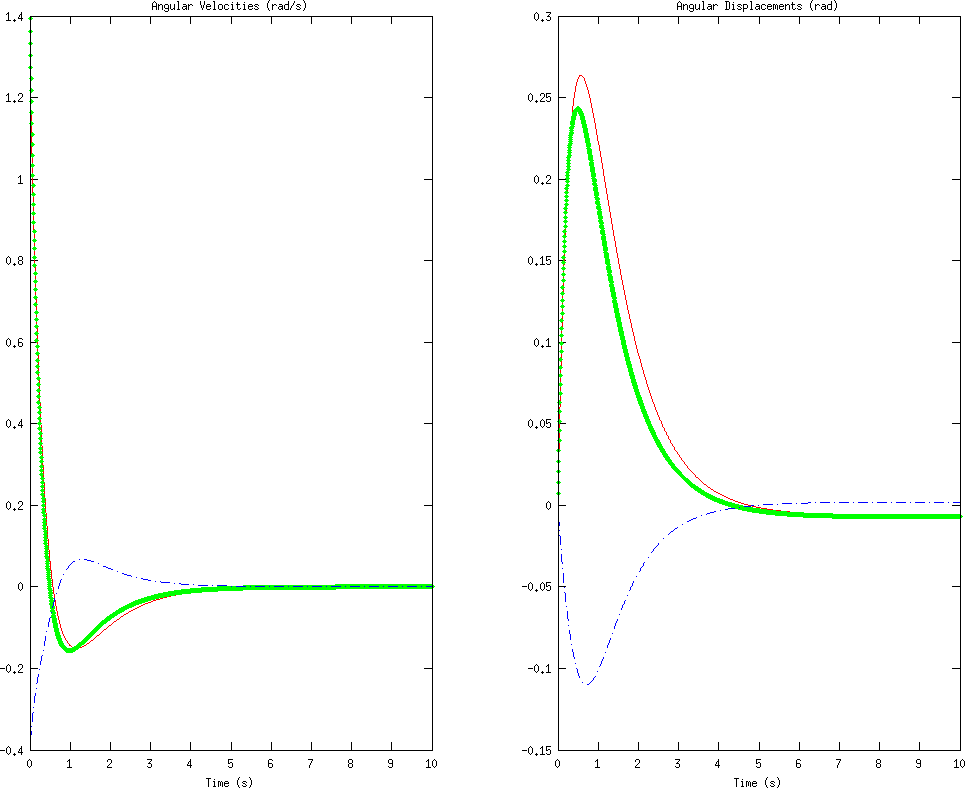
\includegraphics[scale=0.9]{images/pd_controller.png} \\
    {
        Left: Angular velocities. Right: angular displacements. $\phi$, $\theta$, $\psi$ are coded as red, green, and blue.
    }
\end{center}
However, note that the angles are not completely driven to zero. The average steady state error
(error after 10 seconds of simulation) is approximately 0.3$^\circ$. This is a common problem with
using PD controllers for mechanical systems, and can be partially alleviated with a PID controller,
as we will discuss in the next section.

In addition, note that since we are only controlling angular velocities, our positions and linear velocities do
not converge to zero. However, the $z$ position will remain constant, because we have constrained
the total vertical thrust to be such that it keeps the quadcopter perfectly aloft, without ascending
or descending. However, this is really nothing more than a curiosity. With the limited sensing that we have
available to us, there is nothing we can do to control the linear position and velocity of the
quadcopter. While in theory we could compute the linear velocities and positions from the angular
velocities, in practice the values will be so noisy as to be completely useless. Thus, we will
restrict ourselves to just stabilizing the quadcopter angle and angular velocity. (Traditionally,
navigation is done by a human, and stabilization is there simply to make control easier for the
human operator.)

\newpage
We have implemented this PD control for use in our simulation. The controller is implemented as a
function which is given some state (corresponding to controller state, not system state) and the
sensor inputs, and must compute the inputs $\gamma_i$ and the updated state. The code for a PD
control follows.
\begin{minted}{matlab}
% Compute system inputs and updated state.
% Note that input = [$\gamma_1$, $\ldots$, $\gamma_4$]
function [input, state] = pd_controller(state, thetadot)
    % Controller gains, tuned by hand and intuition.
    Kd = 4;
    Kp = 3;

    % Initialize the integral if necessary.
    if ~isfield(state, 'integral')
        params.integral = zeros(3, 1);
    end

    % Compute total thrust
    total = state.m * state.g / state.k / (cos(state.integral(1)) * cos(state.integral(2)));

    % Compute errors
    e = Kd * thetadot + Kp * params.integral;

    % Solve for the inputs, $\gamma_i$
    input = error2inputs(params, accels, total);

    % Update the state
    params.integral = params.integral + params.dt .* thetadot;
end
\end{minted}

\subsection*{PID Control}
PD controllers are nice in their simplicity and ease of implementation, but they are often
inadequate for controlling mechanical systems. Especially in the presence of noise and disturbances,
PD controllers will often lead to steady state error. A PID control is a PD control with another
term added, which is proportional to the integral of the process variable. Adding an integral term
causes any remaining steady-state error to build up and enact a change, so a PID controller should be able to track our
trajectory (and stabilize the quadcopter) with a significantly smaller steady-state error. The equations remain identical
to the ones presented in the PD case, but with an additional term in the error:
\begin{align*}
    e_\phi &= K_d\dot\phi + K_p \int_0^T\dot\phi\dd t + K_i \int_0^T\int_0^T\dot\phi\dd t\dd t \\
    e_\theta &= K_d\dot\theta + K_p \int_0^T\dot\theta\dd t + K_i \int_0^T\int_0^T\dot\theta\dd t\dd t \\
    e_\psi &= K_d\dot\psi + K_p \int_0^T\dot\psi\dd t + K_i \int_0^T\int_0^T\dot\psi\dd t\dd t \\
\end{align*}
However, PID controls come with their own shortcomings. One problem that commonly occurs with a PID control is known as integral windup. 
\begin{center}
    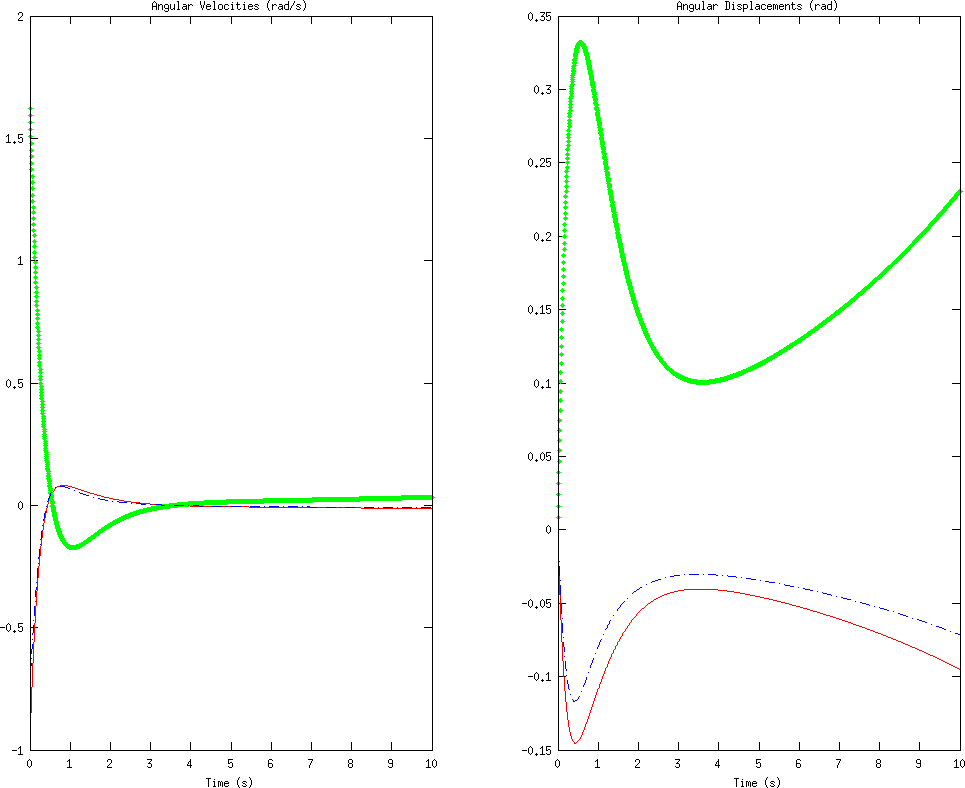
\includegraphics[scale=0.9]{images/windup.png} \\
    {
        In some cases, integral wind-up can cause lengthy oscillations instead of settling. In other cases,
        wind-up may actually cause the system to become unstable, instead of taking longer to reach
        a steady state.
    }
\end{center}
If there is a large disturbance in the process variable, this large disturbance is integrated over time, becoming a still
larger control signal (due to the integral term). However, even once the system stabilizes, the integral is still large, thus
causing the controller to overshoot its target. It may then begin a series of dieing down
oscillations, become unstable, or simply take an incredibly long time to reach a steady state. In order to avoid this, we disable the integral function until we reach
something close to the steady state. Once we are in a controllable region near the desired steady
state, we turn on the integral function, which pushes the system towards a low steady-state error.
\begin{center}
    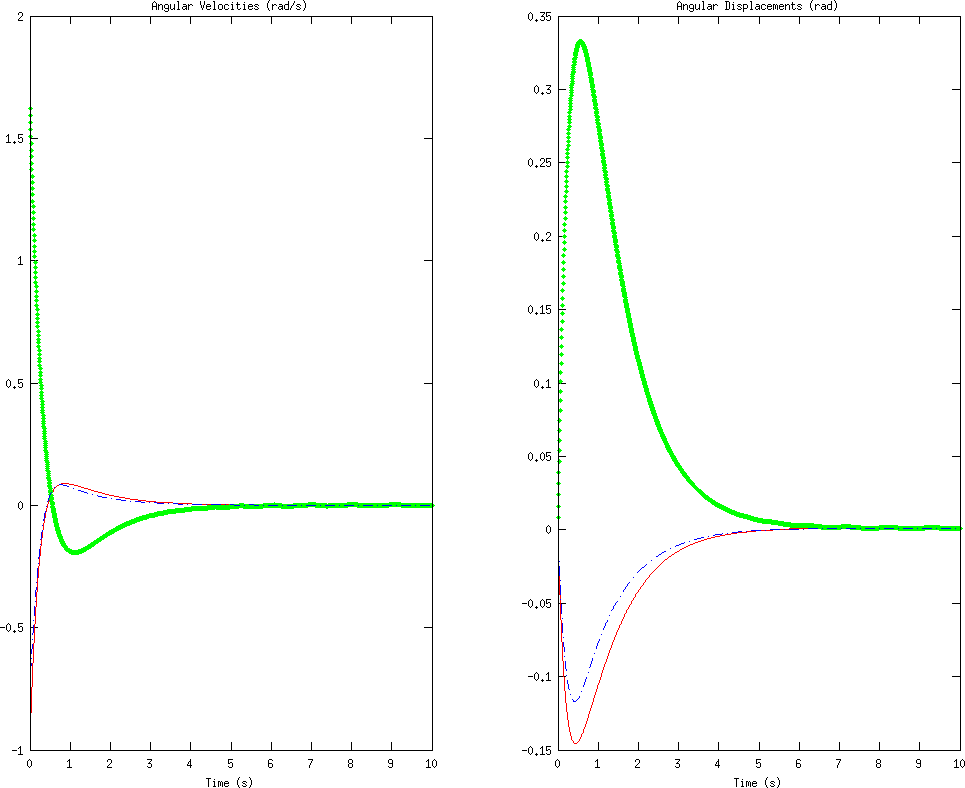
\includegraphics[scale=0.9]{images/pid_controller.png} \\
    {
        With a properly implemented PID, we achieve an error of approximately 0.06$^\circ$ after 10 seconds.
    }
\end{center}
We have implemented this PID control for use in simulation, in the same way as with the PD
controller shown earlier. Note that there is an additional parameter to tune in a PID. The
disturbances used for all the test cases are identical, shown to compare the controllers.
\begin{minted}{matlab}
% Compute system inputs and updated state.
% Note that input = [$\gamma_1$, $\ldots$, $\gamma_4$]
function [input, state] = pid_controller(state, thetadot)
    % Controller gains, tuned by hand and intuition.
    Kd = 4;
    Kp = 3;
    Ki = 5.5;

    % Initialize the integral if necessary.
    if ~isfield(state, 'integral')
        params.integral = zeros(3, 1);
        params.integral2 = zeros(3, 1);
    end

    % Prevent wind-up
    if max(abs(params.integral2)) > 0.01
        params.integral2(:) = 0;
    end

    % Compute total thrust
    total = state.m * state.g / state.k / (cos(state.integral(1)) * cos(state.integral(2)));

    % Compute errors
    e = Kd * thetadot + Kp * params.integral - Ki * params.integral2;

    % Solve for the inputs, $\gamma_i$
    input = error2inputs(params, accels, total);

    % Update the state
    params.integral = params.integral + params.dt .* thetadot;
    params.integral2 = params.integral2 + params.dt .* params.integral;
end
\end{minted}
\pagebreak

\subsection*{Automatic PID Tuning}
Although PID control has the potential to perform very well, it turns out that the quality of the
controller is highly dependent on the gain parameters. Tuning the parameters by hand may be quite
difficult, as the ratios of the parameters is as important as the magnitudes of the parameters
themselves; often, tuning parameters requires detailed knowledge of the system and an understanding
of the conditions in which the PID control will be used. The parameters we chose previously were
tuned by hand for good performance, simply by running simulations with many possibly disturbances
and parameter values, and choosing something that worked reasonably well. This method is clearly
suboptimal, not only because it can be very difficult and labor-intensive (and sometimes more or
less impossible) but also because the resulting gains are not in any way guaranteed to be optimal or
even close to optimal.

Ideally, we would be able to use an algorithm to analyze a system and output the ``optimal'' PID
gains, for some reasonable definition of optimal. This problem has been studied in depth, and many
methods have been proposed. Many of these methods require detailed knowledge of the system being
modeled, and some rely on properties of the system, such as stability or linearity. The method we
will use for choosing our PID parameters is a method known as \emph{extremum seeking}.

Extremum seeking works exactly as the name implies. We define the ``optimal'' set of parameters as
some vector $\vec \theta = (K_p, K_i, K_d)$ which minimizes some cost function $J(\vec\theta)$. In our case, we would
like to define a cost function that penalizes high error and error over extended durations of time.
One candidate cost function is given by
\[J(\vec\theta) = \inv{t_f - t_o} \int_{t_0}^{t_f} e(t, \vec\theta)^2 \dd t\]
where $e(t, \vec\theta)$ is the error in following some reference trajectory with some initial
disturbance using a set of parameters $\vec\theta$. Suppose we were able to somehow compute the
gradient of this cost function, $\nabla J(\vec\theta)$. In that case, we could iteratively improve
our parameter vector by defining a parameter update rule
\[\vec\theta(k + 1) = \vec\theta(k) - \alpha \nabla J(\vec \theta)\]
where $\vec\theta(k)$ is the parameter vector after $k$ iterations and $\alpha$ is some step size
which dictates how much we adjust our parameter vector at each step of the iteration. As
$k\to\infty$, the cost function $J(\vec\theta)$ will approach a local minimum in the space of PID
parameters. 

The question remains as to how we can estimate $\nabla J(\vec\theta)$. By definition,
\[\nabla J(\vec\theta) = \left(\p{ }{K_p} J(\vec\theta), \p{ }{K_i} J(\vec\theta), \p{ }{K_d}
    J(\vec\theta)\right).\]
We  know how to compute $J(\vec\theta)$. Using this, we can approximate the derivative with respect
to any of the gains numerically, simply by computing
\[\p{ }{K} J(\vec\theta) \approx \frac{J(\vec\theta + \delta\cdot \hat{u}_K) - J(\vec\theta-
    \delta\cdot \hat{u}_K)}{2\delta}\] 
where $\hat{u}_K$ is the unit vector in the $K$ direction. As $\delta\to 0$, this approximation
becomes better. Using this approximation, we can minimize our cost function and achieve locally
optimal PID parameters. We can start with randomly initialized positive weights, disturb the system
in some set manner, evaluate $J(\vec\theta)$ by simulating the system for different PID parameters,
and then compute the gradient. Then, using the method of gradient descent, we can iteratively
oprtimize our gains until we have some form of convergence.

The gradient descent method does, however, have several problems. First of all, although it finds a
local minimum, that minimum is only guaranteed to be a \emph{local} minimum - there may be other
minima which are better global minima. In order to avoid choosing suboptimal local minima in the
cost function, we repeat our optimization several times, and choose the best result. We initialize
our PID parameters randomly, so each time we run the optimization we will get a different result. In
addition, instead of choosing disturbance and then optimizing the response to that disturbance, we
use several random disturbances at each iteration and use the average response to compute costs and
gradients. This ensures that our parameters are general and not optimized for a specific
disturbance. In addition, we vary the step size and the number of disturbances to try per iteration,
in order to increase the sensitivity of our results as our iteration continues. We stop iterations
when we detect a steady state, which we do by computing a linear regression on the most recent costs
and iterating until the slope is statistically indistinguishable from zero using a 99\% confidence
interval.

Using our quadcopter simulation, we can define a function that computes the cost for a given set of
PID parameters.
\begin{minted}{matlab}
function J = cost(theta)
    % Create a controller using the given gains.
    control = controller('pid', theta(1), theta(2), theta(3));

    % Perform a simulation.
    data = simulate(control);

    % Compute the integral, $\frac{1}{t_f - t_0} \int_{t_0}^{t_f} e(t)^2 dt$
    t0 = 0;
    tf = 1;
    J = 1/(tf - t0) * sum(data.theta(data.t >= t0 & data.t <= tf) .^ 2) * data.dt;
end
\end{minted}
We can use this function to approximate a derivative with respect to a gain:
\begin{minted}{matlab}
% Compute derivative with respect to first parameter.
delta = 0.01;
var = [1, 0, 0];
derivative = (cost(theta + delta * var) - cost(theta - delta * var)) / (2 * delta);
\end{minted}
We can then use our gradient descent method (with all modifications described above) to minimize the
cost function and obtain a good set of PID parameters. We can verify that our tuning method is
working by visualizing the cost function versus the iteration number, and seeing that the cost
function is indeed going down and stabilizing at a local minimum.
\begin{center}
    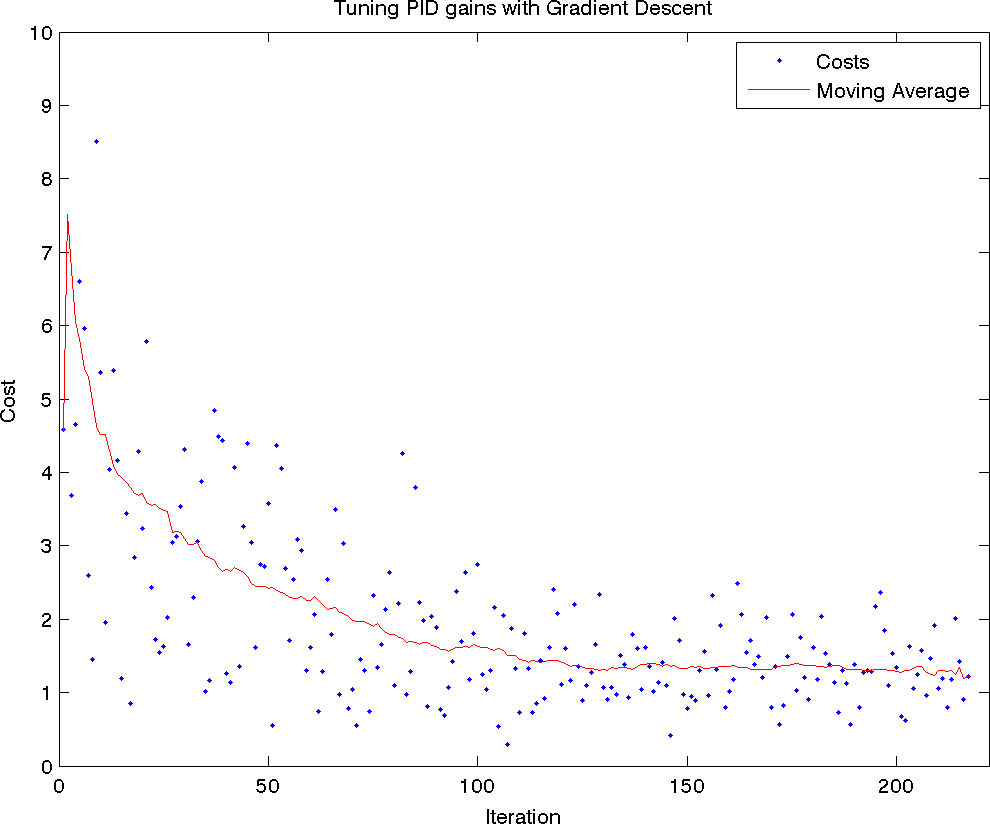
\includegraphics[scale=0.60]{images/training.png} \\
    {
        Cost function plotted as a function of iteration number, along with moving average. 
        Tuning stops when the slope of the moving average becomes statistically indistinguishable
        from zero with a 99\% confidence interval.
    }
\end{center}
We can compare the manually-chosen PID parameters with those designed by the algorithm. 
\begin{center}
    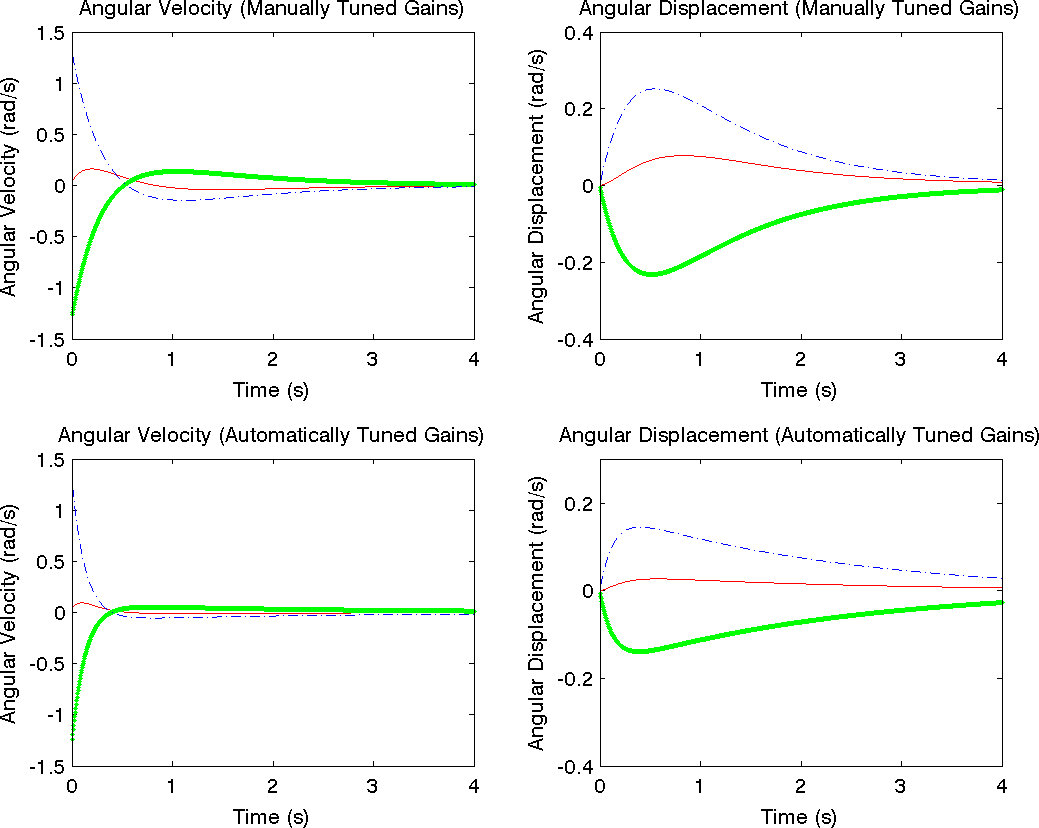
\includegraphics[scale=0.9]{images/pid_gains_comparison.png} \\
    {
        Top: Angular velocities and angular displacements, using manually tuned PID controller.
        Bottom: Angular velocities and angular displacements, using automatically tuned PID
        controller.
    }
\end{center}
The automatically-chosen PID parameters do significantly better overall. They have significantly
smaller swings in value, overshoot significantly less, and converge faster. However, the error in
the angular displacement takes longer to converge to zero with the automatically tuned parameters
than with the manually turned parameters, although the initial convergence is much better when the
parameters are chosen via gradient descent. This is due to the fact that our cost function
emphasizes squared error, and thus gives priority to minimizing overall error magnitude rather than
long-term convergence. We could easily modify our cost function to give higher priority to long-term
error, in which case the automatically-tuned parameters are likely to do better.
\newpage

\section*{Conclusion}
We derived equations of motion for a quadcopter, starting with the voltage-torque relation for the
brushless motors and working through the quadcopter kinematics and dynamics. We ignored
aerodynamical effects such as blade-flapping and non-zero free stream velocity, but included air
friction as a linear drag force in all directions. We used the equations of motion to create a
simulator in which to test and visualize quadcopter control mechanisms.

We began with a simple PD controller. Although the PD controller worked, it left a significant
steady-state error. In order to decrease the steady-state error, we added an integral term in order
to create a PID controller. We tested the PID controller (with minor modifications to prevent
integral wind-up) and found that it was better at preventing steady-state error than the PD
controller when presented with the same disturbances and using the same proportional and derivative
gains. We also found that tuning the PID controller was difficult, and would often lead to an
unstable system for unknown reasons. In order to avoid the difficulty of PID tuning and find the
optimal set of parameters, we used a gradient-descent based extremum seeking method in order to
numerically estimate gradients of a cost function in PID-parameter space and iteratively choose a
set of parameters to minimize the cost function. We found that the resulting controller was
significantly better than the one using manually turned parameters.

\end{document}
